\begin{exercise}{%
    Határozzuk meg az alábbi függvény abszolút szélsőértékeit az adott halmazokon!
  }
  \[
    f(x; y) = 3x + 4y
  \]
  \begin{enumerate}[a)]
    \item $H = {(x;y) : x^2 + y^2 \leq 4}$
    \item $H = {(x;y) : x^2 + y^2 \leq 4, y \geq 0}$
  \end{enumerate}

  \exsol[20.75cm]{
    \begin{enumerate}[a)]
      \item $H = {(x;y) : x^2 + y^2 \leq 4}$\\[2mm]
            %
            Gondolkodós megoldás: A gradiens kijelöli számunkra a függvény
            legnagyobb növekményének irányát:
            \[
              \grad f(x;y) = \begin{bmatrix}
                3 \\ 4
              \end{bmatrix}
              \text.
            \]
            Normáljuk a függvény gradiensét:
            \[
              \uvec v = \frac{1}{\sqrt{3^2 + 4^2}} \begin{bmatrix}
                3 \\ 4
              \end{bmatrix} = \begin{bmatrix}
                3/5 \\ 4/5
              \end{bmatrix}
              \text.
            \]
            A szélsőértékeket a 2 egység sugarú körön belül keressük. Mivel a
            függvény képe egy sík ezért a teljes értelmezési tartományán
            szélsőértékei nincsenek. A szélsőértékek ezért biztosan a tartomány
            peremén fognak elhelyezkedni. A maximum hely helyvektora:
            $2 \uvec v$, a minimum helyé pedig: $-2 \uvec v$. Az adott halmazon
            vett maximum és minimum:
            \[
              f(6/5; 8/5) = 10
              \text,\qquad
              f(-6/5; -8/5) = -10
              \text.
            \]

            Számolósabb megoldás: Lagrange-multiplikátor segítségével.
            Ekkor az alábbi függvénynek keressük a szélsőértékeit:
            \[
              F(x; y; \lambda) = 3x + 4y + \lambda (x^2 + y^2 - 4)
            \]
            Határozzuk meg a parciális deriváltakat:
            \[
              \pdv{F}{x} = 3 + 2x \lambda = 0
              \text, \qquad
              \pdv{F}{y} = 4 + 2y \lambda = 0
              \text, \qquad
              \pdv{F}{\lambda} = x^2 + y^2 - 4 = 0
              \text.
            \]
            Az első és a második egyenlet alapján:
            \[
              x = \frac{-3}{2\lambda}
              \text, \qquad
              y = \frac{-4}{2\lambda}
              \text.
            \]
            Ezek segítségével a harmadik egyenlet:
            \[
              \frac{9}{4\lambda^2} + \frac{16}{4\lambda^2} - 16 = 0
              \quad \rightarrow \quad
              \lambda_{12} = \pm \frac{5}{4}
              \text.
            \]
            A keresett pontok tehát:
            \[
              (x_1; y_1) = (3/5; 4/5)
              \text, \qquad
              (x_2; y_2) = (-3/5; -4/5)
              \text.
            \]
            A függvényértékek pedig:
            \[
              f(6/5; 8/5) = 10
              \text,\qquad
              f(-6/5; -8/5) = -10
              \text.
            \]
            Látható, hogy ezzel a módszerrel is ugyan azt a megoldást kaptuk.

      \item $H = {(x;y) : x^2 + y^2 \leq 4, y \geq 0}$\\[2mm]
            %
            Gondolkodós megoldás: Most is a gradienst fogjuk segítségül hívni.
            Mivel a függvény képe továbbra is egy sík, ezért a szintvonalai a
            gradiensre merőleges egyenesek lesznek.
            \begin{center}
              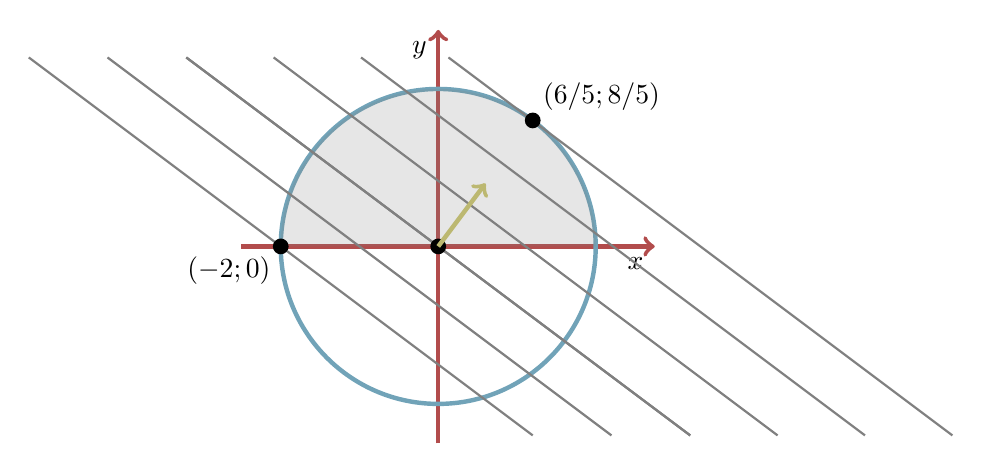
\begin{tikzpicture}[thick]
                \draw[-to, draw=red!40!gray, ultra thick]
                (-2.5, 0) -- (2.75, 0) node[below left] {$x$};
                \draw[-to, draw=red!40!gray, ultra thick]
                (0, -2.5) -- (0, 2.75) node[below left] {$y$};

                \draw[draw=cyan!40!gray, ultra thick] (0,0) circle (2);
                \fill[gray, opacity=.2] (2,0) arc [
                    start angle=0,
                    end angle=180,
                    x radius=2cm,
                    y radius=2cm,
                  ];
                \foreach \s in {-2,-1,...,0}{
                    \draw[
                      xshift=\s*1cm,
                      gray,
                    ](-3.2,2.4) -- (3.2,-2.4);
                  }
                \foreach \s in {0,1,...,3}{
                    \draw[
                      xshift=\s*1.11cm,
                      gray,
                    ](-3.2,2.4) -- (3.2,-2.4);
                  }

                \fill (0,0) circle (.1);
                \fill (-2,0) circle (.1) node[below left] {$(-2;0)$};
                \fill (1.2,1.6) circle (.1) node[above right] {$(6/5;8/5)$};;

                \draw[ultra thick, -to, yellow!40!gray] (0,0) -- (.6,.8);
              \end{tikzpicture}
            \end{center}
            Az ábra alapján a maximum és minimum:
            \[
              f(6/5; 8/5) = 10
              \text,\qquad
              f(-2; 0) = -6
              \text.
            \]

            Számolásos megoldás: Az előző részfeladatban kapott eredmények
            közül a maximum itt is helyt áll, viszont a minimumot az adott
            egyenes és a kör metszéspontjaiban kell keresnünk. Kettő
            multiplikátort kell bevezetnünk:
            \[
              F(x; y; \lambda; \mu) = 3x + 4y + \lambda (x^2 + y^2 - 4) + \mu (y)
            \]
            Határozzuk meg a parciális deriváltakat:
            \[
              \pdv{F}{x} = 3 + 2x \lambda = 0
              \text, \quad
              \pdv{F}{x} = 4 + 2y \lambda + \mu = 0
              \text, \quad
              \pdv{F}{\lambda} = x^2 + y^2 - 4 = 0
              \text, \quad
              \pdv{F}{\mu} = y = 0
              \text.
            \]
            A lehetséges szélsőérték helyek:
            \[
              f(-2;0) = -6
              \text,
              \qquad
              f(2;0) = 6
              \text.
            \]
            A tartományon a függvény maximuma és minimuma tehát:
            \[
              f(6/5; 8/5) = 10
              \text,\qquad
              f(-2; 0) = -6
              \text.
            \]
            Látható, hogy itt is mind a két módszerrel ugyan azt a megoldást
            kaptuk eredményül.
    \end{enumerate}
  }
\end{exercise}
